% interactnlmsample.tex
% v1.05 - August 2017

\documentclass[]{interact}

\usepackage{epstopdf}% To incorporate .eps illustrations using PDFLaTeX, etc.
\usepackage[caption=false]{subfig}% Support for small, `sub' figures and tables
%\usepackage[nolists,tablesfirst]{endfloat}% To `separate' figures and tables from text if required
%\usepackage[doublespacing]{setspace}% To produce a `double spaced' document if required
%\setlength\parindent{24pt}% To increase paragraph indentation when line spacing is doubled

\usepackage[numbers,sort&compress]{natbib}% Citation support using natbib.sty
\bibpunct[, ]{[}{]}{,}{n}{,}{,}% Citation support using natbib.sty
\renewcommand\bibfont{\fontsize{10}{12}\selectfont}% Bibliography support using natbib.sty
\makeatletter% @ becomes a letter
\def\NAT@def@citea{\def\@citea{\NAT@separator}}% Suppress spaces between citations using natbib.sty
\makeatother% @ becomes a symbol again

\usepackage[utf8]{inputenc}
\usepackage{url}
\usepackage{graphicx}
\graphicspath{{images/}}
\usepackage{csquotes}
\usepackage{booktabs}
\usepackage{array}
\usepackage{amssymb}
\usepackage{tabularray}
\usepackage{tabularx}
\usepackage{makecell}
\usepackage[title]{appendix}

\usepackage{pdflscape}
\usepackage{afterpage}

\theoremstyle{plain}% Theorem-like structures provided by amsthm.sty
\newtheorem{theorem}{Theorem}[section]
\newtheorem{lemma}[theorem]{Lemma}
\newtheorem{corollary}[theorem]{Corollary}
\newtheorem{proposition}[theorem]{Proposition}

\theoremstyle{definition}
\newtheorem{definition}[theorem]{Definition}
\newtheorem{example}[theorem]{Example}

\theoremstyle{remark}
\newtheorem{remark}{Remark}
\newtheorem{notation}{Notation}

\newcommand{\tc}{T$_{c}$}
\providecommand{\keywords}[1]


\begin{document}

\articletype{RESEARCH PAPER}% Specify the article type or omit as appropriate

\title{Automatic Extraction of Materials and Properties from Superconductors Scientific Literature}

\author{
    \name{Luca Foppiano\textsuperscript{a}\thanks{Corresponding authors: Luca Foppiano (luca@foppiano.org) and Masashi Ishii (ISHII.Masashi@nims.go.jp)}, Pedro Baptista de Castro\textsuperscript{b}, Pedro Ortiz Suarez\textsuperscript{c}, Kensei Terashima\textsuperscript{b}, Yoshihiko Takano\textsuperscript{b}, Masashi Ishii\textsuperscript{a}}
    \affil{\textsuperscript{a}Material Database Group, MaDIS, NIMS, Tsukuba, JP; \textsuperscript{b}Nano Frontier Superconducting Materials Group, MANA, NIMS, Tsukuba, JP; \textsuperscript{c}Data and Web Science Group, University of Mannheim, Mannheim, DE}
}


\maketitle

\begin{abstract}
The automatic extraction of materials and related properties from the scientific literature is getting more attention in data-driven materials science (Materials Informatics).
In this paper, we discuss grobid-superconductors, our solution for automatically extract superconductor material names and respective properties from text.
Built as Grobid module it combines Machine Learning and Heuristic approaches in a multi-step  architecture supporting input data as raw text or PDF documents.
Using grobid-superconductors, we built SuperCon\textsuperscript{2}, a database of 40324 materials-properties records from 37700 papers.
The material (or sample) information is represented by name, chemical formula, material class, and is characterised by shape, doping, variables for components, substrate as adjoined information.
The properties include the T\textsubscript{c} superconducting critical temperature and, when available, applied pressure with T\textsubscript{c} measurement method.
\end{abstract}

\begin{keywords}
materials informatics, superconductors, machine learning, nlp, tdm
\end{keywords}

\begin{quote}
\textbf{CLASSIFICATION}: Machine learning, Text mining, NLP
\end{quote}


\section{Introduction}
In recent years, with the creation of computational databases, such as the Materials Project (MP)~\cite{materialsprojectJain2013}, the Open Quantum Materials Database (OQMD)~\cite{oqmdkirklin2015open}, and then experimental data repositories such as NIMS MDR (\url{http://mdr.nims.go.jp})~\cite{ranganathan_anusha_2019_3553963}, the focus has been steadily shifting towards a data-driven design of materials which is often called as Materials Informatics (MI). 
Such an approach is expected to accelerate the exploration of functional materials, as it does not rely on the intuition of very little genius researchers nor on their limited experience.
In this new paradigm, the efficient use of data to guide experiments and materials property prediction through the use of machine learning methods takes the centre stage. 
For example, data-driven methods have been used to search/design magneto-caloric materials~\cite{Bocarsly2017,Castro2020-12,court2021inverse}, photo-catalysts for hydrogen splitting~\cite{xiong2021optimizing}, thermoeletrics~\cite{iwasaki2019machine}, and superconductors~\cite{stanev_machine_2017}. 
In such a data-driven search, one of the most important keys lies in the availability of the data, that at least should consist of compositions of materials and their physical properties. 
In the specific case of superconductivity, most of the data-driven works~\cite{stanev_machine_2017, le2020critical,Hamlin2019SuperconductivityNR} relies on a single database: SuperCon (\url{http://supercon.nims.go.jp}). 

SuperCon is a structured database of superconductors materials and properties, developed at the National Institute for Materials Science (NIMS) in Japan. 
At the time of writing this paper, SuperCon contains about 33000 inorganic and 600 organic materials and is the ``de-facto'' standard in data-driven research for superconductors materials  (about 4400 articles contain the mention ``\textit{supercon database}'' in Google Scholar). 
However, SuperCon harvesting process is currently fully manual ``from scratch'': the humans have to read the human-readable printed matter such as PDF documents and enter the information in the system. 
The efficiency is directly proportional to the number of available human curators.
Considering the cost of database construction, it is necessary to consider an assisted or alternative system that improves throughput while ensuring data quality equivalent to that of manual extraction.

As a solution, we are developing a hybrid data extraction methods from scientific literature combining automation using text data mining and manual curation.
The automated system extracts and formats potential data and proposes them to the curator as ``pre-cooked'' structured data: (a) Highlight the relevant entities on the original document. 
(b) Pre-fill the extracted information in a tabular format.
% By linking (a) highlighted source text and (b) structured information, curators can quickly move back and forth between (a) and (b). 
In building the automatic part of this hybrid system (training, evaluation) we used SuperMat~\cite{foppiano2021supermat}, which we recently constructed. 
% This is a dataset linked to data annotated against the full text of the scientific literature on superconductivity research. 
% We used SuperMat not only as training data for machine learning, but also for NLP evaluation.

% 6. in this work we present X, where we did Y and obtain Z
In this work, we present \textit{grobid-superconductors}: a system to extract automatically structured information of superconductors materials and properties from scientific literature. 
The tool is a specialised module of Grobid~\cite{GROBID}, a machine learning library designed to parse and structure scientific documents. 
Grobid provides an open source platform for building specialised modules: astronomical entities recognition\cite{grobid-astro}, dictionaries~\cite{khemakhem:hal-01508868}, software mentions~\cite{lopez2021mining}, and physical measurements extraction~\cite{foppiano2019quantities}.
Grobid provides several built-in features including access to PDF document layout information, citation resolution, bibliographic information consolidation through \textit{biblio-glutton}~\cite{biblio-glutton-lookup} a fast open-source reference matching service for CrossRef data, and a diverse set of ML architectures from a fast linear Conditional Random Field (CRF) to the latest state-of-the-art deep learning implementations.

% 7. what is our purpose? 
Using grobid-superconductors and other sub-tools, we established a pipeline for processing a large number of documents and obtaining an automated database of superconductors materials and properties. 
We processed 37770 papers from ArXiv (\url{https://arxiv.org}) and obtained a database of 40324 records. 
This new database, named SuperCon\textsuperscript{2}, can become the automated staging area for SuperCon, bridged by a curation interface. 
The project was also an opportunity to focus on properties that gained interest in recent scientific trends and that are underrepresented in SuperCon. 
The ``pressure'' applied to obtain superconductivity (about 20 records in Supercon), has gained attention because it can change radically the physical structure of a material.
The ``method'' used to measure the superconducting transition temperature \tc~(about 600 records in SuperCon) can be used to semantically recognise multiple \tc s obtained from the same material or sample (e.g. distinguish calculated and experimental \tc). 

\section{Grobid-superconductors}

% Overview from the other paper, what are the differences and some repetition on the previous paper 
\textit{Grobid-superconductor} is a web application for processing text or PDF documents to extract materials and corresponding properties. 
We develop \textit{grobid-superconductors} as a \textit{Grobid} library~\cite{GROBID} module following some principles (multi-step, sentence-based, fulltext-based) discussed in a previous preliminary study~\cite{foppiano:hal-02870896}.  
\textit{Grobid} brings several advantages: a) It integrates with \textit{pdfalto}\footnote{\url{https://github.com/kermitt2/pdfalto}}, a specialised tool for converting PDF to XML which mitigates extraction issues such as the resolution of embedded fonts, invalid character encoding, and the reconstruction of the correct reading order.
b) It allows access to PDF document layout information for both machine learning and document decoration (e.g. coordinates in the PDF document) and, finally, c) it provides access to a set of high-quality, pre-trained machine learning models for structuring documents.
\textit{Grobid-superconductors} is structured as a three-steps process as illustrated in Figure~\ref{fig:pipeline-overview} and described in the following sections~\ref{subsubsec:document-structuring},~\ref{subsubsec:extraction}, and~\ref{subsubsec:linking}.

\begin{figure}[ht]
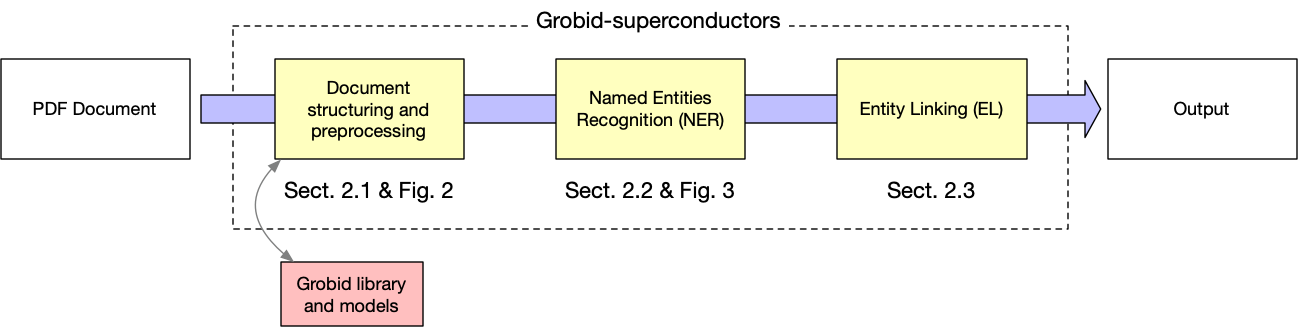
\includegraphics[width=\textwidth]{schema-architecture-colors}
\caption{Processing pipeline for extracting superconductors materials and properties. }
\label{fig:pipeline-overview}
\end{figure}

\paragraph*{Abstract versus fulltext}
At the time of writing this paper, we are aware of related works that utilise text from abstracts as training data for machine learning. 
The main reason is that abstracts are usually freely available as text~\cite{kononova_text-mined_2019}, and contain condensed information~\cite{yamaguchi-etal-2020-sc, court_magnetic_2020}. 
Accurately parsing the full text presents more challenges, however, they are mitigated by the \textit{Grobid} library and the full texts contain a broader range of information, including the sample preparation process, negative results (e.g. absence of superconductivity for certain samples), and background information (e.g. report on other materials from referenced works). 
% Such examples are needed to supply knowledge of non-superconductivity when building a superconductors prediction model~\cite{stanev_machine_2017}. 
Thus, \textit{grobid-superconductors} is built to support full-text documents. 

% Sentences vs Paragraphs 
\paragraph*{Paragraphs versus sentences}
Another question related to NLP processing is whether to use sentence-based or paragraph-based text. 
While paragraphs can be extracted as part of the layout of PDF documents, obtaining sentences adds an additional step which processes text using a sentence segmenter.
However, sentences are smaller by definition (English writing guidelines recommend less than 25 words) and in deep learning, this brings some advantages. 
In training and prediction, sentences will likely be shorter than the ``max sequence length'' limitation (e.g. 512 tokens for transformers).
During training sentences also use less memory and let us train models with a larger ``batch size'', which has been shown to provide better results~\cite{roberta}.
%, and c) SciBERT~\cite{Beltagy2019SciBERT} models are pre-trained on sentences while RoBERTa~\cite{roberta} models are pre-trained with splitting paragraphs.

We decided to use sentence-based text in \textit{grobid-superconductors} after performing experiments on a smaller scale, applied to our tasks. 
For the NER tasks, we trained and evaluated a sequence labelling model for each version (paragraphs-based and sequence-based) on four annotated documents (3/1 documents partition for training/evaluation) from SuperMat~\cite{foppiano2021supermat}.
As indicated in Table~\ref{tab:comparison-evaluation-sentences-paragraphs}, the F1-score increase by 17.94 points \% by using sentence-based text.
% Our intuition suggests that this improvement can be mainly explained by the increase in the number of training examples for the same amount of text.

\begin{table}[ht]
\centering\small
\begin{tabular}{lrrr}
\toprule
\textbf{Label} & \textbf{Precision} & \textbf{Recall} & \textbf{F1} \\
\midrule
Paragraph-based micro avg. & 44.44 & 27.21 & 33.76   \\
Sentence-based micro avg. & 48.41 & 50.00 & 51.70  \\
\bottomrule
\end{tabular}
\caption{\label{tab:comparison-evaluation-sentences-paragraphs} Results from cross-validation using sentence-based or paragraphs based.  }
\end{table}

In the Linking task we want to maximise precision. 
In our previous work~\cite{foppiano2019proposal} we noticed that limiting linking entities within the same sentence (versus paragraphs) would obtain higher precision (68.7\% versus 57\%) at the expense of lower recall (6.5\% versus 10.7\%), and F1-score (11.87\% versus 18.01\%). 
In both our tasks we found evidence that a sentence-based dataset is more beneficial than paragraph-based dataset.


\subsection{Document structuring and pre-processing}
\label{subsubsec:document-structuring}
In the first step of our process, the PDF document is converted into an internal model based on a list of text statements, tokens, and features.
The input document is processed using the Grobid original models where we apply customised processes for document header and content. 
We select a subset of bibliographic information from the header: title, authors, DOI, publisher, journal, and year of publication and we consolidate them via Grobid to match the publisher's quality (even by processing the ``preprint version'' of the publication). 
The superconductors entities extraction is applied to the content, only on relevant text items: title, abstract, text content from body or annexe, text content from figure and table captions (Figure~\ref{fig:grobid-document-processing}).

\begin{figure}[ht]
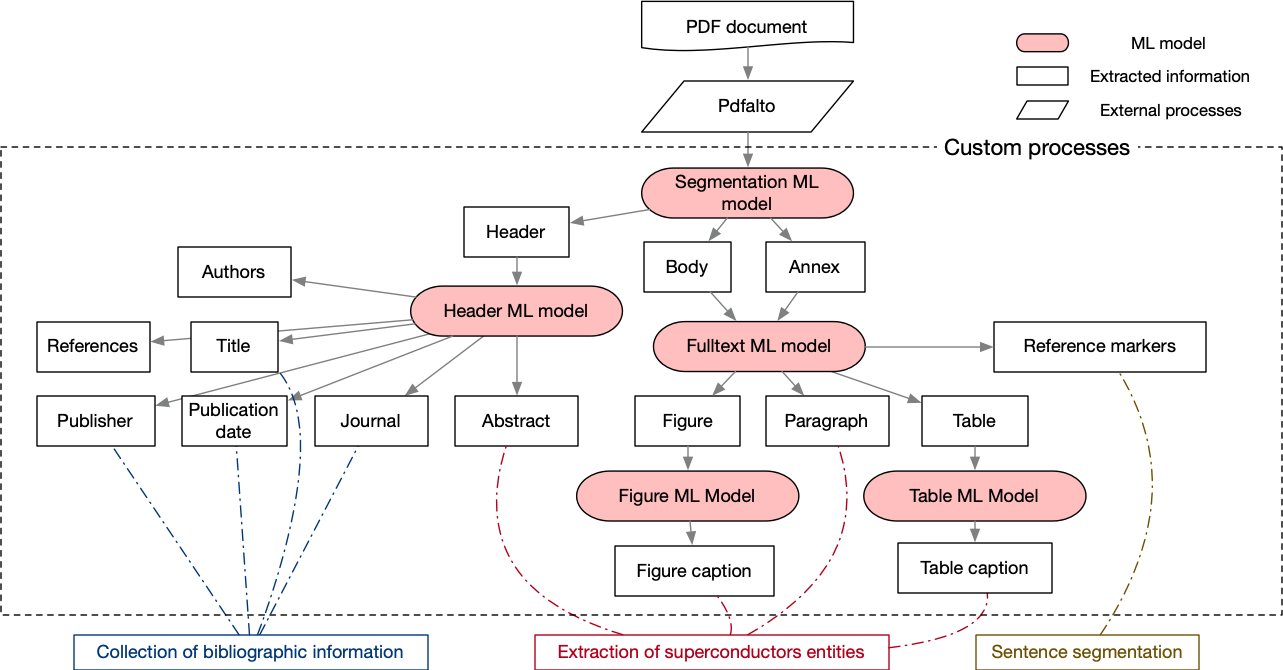
\includegraphics[width=\textwidth]{document-structuring-colors}
\caption{Grobid-superconductors extraction processes (bibliographic information, superconductors entities extraction and sentence segmentation) within the Grobid cascade data flow.}
\label{fig:grobid-document-processing}
\end{figure}

We use the collected reference markers (also called \textit{reference callout}) from text as features for improving the paragraph segmentation in sentences: the segmentation is cancelled if the ``end of sentence'' falls within the boundaries of a reference marker. 
For example, a sentence containing a reference in the form ``\textit{Foppiano et. al.}'' may be mistakenly segmented at ``\textit{et.}''.

% The main properties are: 
% \begin{itemize}
%     \item \textit{LayoutTokens} stores the layout information of each token: style (italic, bold, superscript, and subscript), font (font type, font size), positions (coordinates (a list of pairs x,y), offset position), 
%     \item \textit{section} and \textit{subsection} are the Grobid main sections: header, body and annex, and the second-level processing (paragraph, table or figure caption, abstract, title), respectively,
%     \item \textit{spans} collects extracted entities including type, attributes (as key-value information), and offsets within text and layout tokens.
% \end{itemize}


\subsection{Entities Extraction}
\label{subsubsec:extraction}

The second step is the \textit{Entities Extraction} performing the Named Entity Recognition (NER) task on previously extracted text. 

\subsubsection*{Overview}

\begin{figure}[ht]
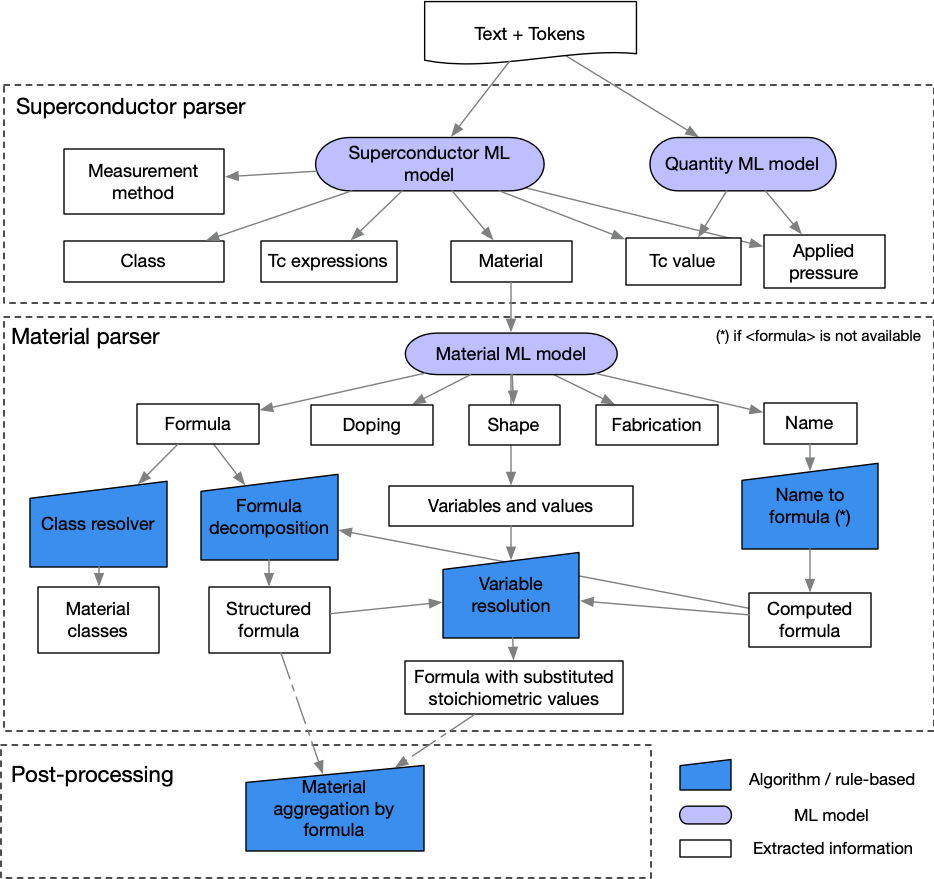
\includegraphics[width=\textwidth]{schema-extraction-colors}
\caption{\label{fig:extraction-ml-models-cascade-architecture} Cascade architecture in the Entities Extraction step. The white rectangles indicate the extracted information (described in Tables~\ref{tab:superconductors-parser-entities} and~\ref{tab:material-parser-entities}). 
The ML models and the rule-based algorithms are identified by light grey and dark grey shapes, respectively.}
\end{figure}

As illustrated in Figure~\ref{fig:extraction-ml-models-cascade-architecture} the ``superconductors parser'' extracts the main superconductors-related information by aggregating the resulting entities from two ML models. 
The \textit{superconductors ML model}, developed based on the SuperMat schema~\cite{foppiano2021supermat}, and the \textit{quantities ML model}, developed in a separated grobid-module for measurement extraction~\cite{foppiano2019quantities} for which we limit the output to only temperatures and pressures.
Overlapping entities are merged: exact duplicates are removed and the largest entities (in terms of string length) are preserved.
The resulting entities are summarised in Table~\ref{tab:superconductors-parser-entities}.

\begin{table}[ht]
\centering\small
\scalebox{0.71}{
\begin{tabular}{m{19em} m{30em}}
\toprule
\textbf{Entity} (\textbf{Tag})& \textbf{Description} \\ 
\midrule
\multicolumn{2}{c}{\textbf{Machine learning}} \\
\midrule
Material (\texttt{<material>}) & Materials and samples names, formulas, including stochiometric formulas, substitution variables of values and elements, shape, doping, substrate \\
Class (\texttt{<class>}) & Groups of materials having similar characteristics or common strategic compounds that define their nature \\
T\textit{c} value (\texttt{<tcValue>})& The value of the superconductors critical temperature\\
T\textit{c} expressions (\texttt{<tc>}) & Expressions in the text that provide information about the phenomenon of superconductivity related to a value, interval or variation of the T\textsubscript{c}\\
Measurement methods (\texttt{<me\_method>}) & Techniques used to measure or calculate the presence of superconductivity. \\
Applied pressure (\texttt{<pressure>}) & Applied pressure when superconductivity is recorded\\
\bottomrule
\end{tabular}
}
\caption{Synthesis of the superconductors parser entities. }
\label{tab:superconductors-parser-entities}
\end{table}

The entities of type \texttt{<material>} are passed in cascade to the ``material parser'' which combines ML and tools to extract further information and structures. 
First, the material raw string is passed through a \textit{material ML model} to segment the raw material string (Table~\ref{tab:material-parser-entities}). 
Then, we apply different processes, based on which information is available: 
\begin{itemize}
    \item formulas are decomposed into a structured composition. We identify each pair of element-stoichiometry (e.g ``O'': 7.0) using mat2chem~\cite{kononova_text-mined_2019} and Pymatgen~\cite{Ong2013}, 
    \item if only the name is available, we obtain the formula (e.g. hydrogen to \textit{H}), 
    \item using heuristics, we classify the formula with tags that follows the superconductors researcher ``material class'' conventions, for example Cuprate, Oxides, Alloys, etc. 
    \item using the variables and values extracted, we substitute them into partial formulas. For example, in \texttt{La 4 Fe 2 A 1-x O 7 (A=Mg,Co; x=0.1,0.2)}, we substitute \textit{A} and \textit{x} using their parsed values, and applying permutations we obtain four \textit{resolved formulas}: \texttt{La 4 Fe 2 Mg 0.9 O 7}, \texttt{La 4 Fe 2 Mg 0.8 O 7}, \texttt{La 4 Fe 2 Co 0.9 O 7}, \texttt{La 4 Fe 2 Co 0.8 O 7}.
\end{itemize}

\begin{table}[ht]
\centering
\scalebox{0.7}{
\begin{tabular}{m{16em} m{30em}}
\toprule
\textbf{Entity} (\textbf{Tag})& \textbf{Description} \\ 
\midrule
Name (\texttt{<name>}) & The canonical name of a material (e.g. Hydrogen, PCCO, Carbon) \\
Formula (\texttt{<formula>}) & Chemical formula of the material (e.g. \texttt{Pr1.869Ce0.131CuO 4-}, \texttt{MgB2}, \texttt{La 2-x Sr x CuO 4}) \\
Doping (\texttt{<doping>})& Doping ratio and doping materials that are adjoined to the material name (e.g. \texttt{Zn-doped}, \texttt{2\% Zn-doped})\\
Shape (\texttt{<shape>}) & shape of the material (e.g. single crystal, polycrystalline, thin film, powder, film) \\
Substitution variables (\texttt{<variable>}) & Variables that can be substituted in the formula. \\
Substitution values (\texttt{<value>}) & Values expressed in the doping. \\
Substrate (\texttt{<substrate>}) & Substrates as defined in the material name \\
Fabrication (\texttt{<fabrication>}) & Represent eventual additional information that are not belonging to any of the previous tags  (e.g. intercalated, electron-doped)\\
\bottomrule
\end{tabular}
}
\caption{\label{tab:material-parser-entities} Synthesis of the material parser entities. }
\end{table}

Finally, after all entities are extracted, the post-processing aggregates different mentions of the same materials using the parsed formulas at document-level. 
For example \texttt{hydrogen} and \texttt{H}, or formula with partial substitutions such as \texttt{La 2 Fe 1-x O 7 (x = 0.1, 0.2)} will be aggregated with materials like \texttt{La 2 Fe 0.9 O 7} appearing in other sections of the same document. 

\subsubsection*{Machine Learning study}

In this section we discuss the novel ML models we have trained for extracting specialised entities: \textit{superconductors ML model} and \textit{material ML model} (Figure~\ref{fig:extraction-ml-models-cascade-architecture}). 
SuperMat~\cite{foppiano2021supermat}, our training dataset, counts 162 papers at the time of writing and is composed of annotated full-text and layout features from PDF documents. 

For both ML models we trained and evaluated these four architecture/implementations: 
\begin{itemize}
    \item Linear CRF (CRF)
    \item Bidirectional LSTM with CRF~\cite{Lample2016NeuralAF} (BidLSTM\_CRF)
    \item Bidirectional LSTM with CRF with Features~\cite{Lample2016NeuralAF} is the same as the previous one with an additional input channel for features (BidLSTM\_CRF\_FEATURES)
    \item SciBERT~\cite{Beltagy2019SciBERT} using a CRF as activation layer (Scibert)
\end{itemize}

The ML models are interfaced by Grobid, which uses the Wapiti\cite{lavergne2010practical} implementation for linear CRF, and DeLFT (Deep Learning For Text)~\cite{DeLFT} for deep learning models.
The architectures CRF and BidLSTM\_CRF\_FEATURES make use of orthogonal features we have summarised in Table~\ref{tab:ML-model-features}. 

\paragraph*{Superconductors ML model}

\subparagraph*{Holdout set}
The holdout set must be balanced and should follow the same distribution of the target dataset. 
We assembled the holdout set by manually selecting from SuperMat 32 documents (24\%) with the same ratio of training examples, entities and unique entities (Figure~\ref{fig:training-holdout-set-distribution}a).
Maintaining the same rate (80/20) for entity type distribution is more challenging: in average, we obtained around 15-18\% of labels of each type in the holdout set (Figure~\ref{fig:training-holdout-set-distribution}b), except for the \texttt{<material>} label (23\%). %(Tables~\ref{tab:training-holdout-set-distribution-annex} and \ref{tab:training-holdout-distribution-labels}). 
The remaining 76\% (132 documents) is used for training. 

We define the ``out-of-domain'' ratio as the number of unique entities from the holdout set that are not in the training set. 
The holdout set ``out-of-domain'' ratio is on average around 72\%, which requires the model to be able to generalise well. 
All the labels have ``out-of-domain'' ratio above 24\%  (Figure~\ref{fig:out-domain-holdout}) with the highest for the \texttt{<material>} at 82\%. The labels \texttt{<me\_method>} have the lowest ``out-of-domain'' ratio at 25\% which can be explained by a high uniqueness of entities (355 entities are reduced to 57 unique). 

\begin{figure}[ht]
\centering
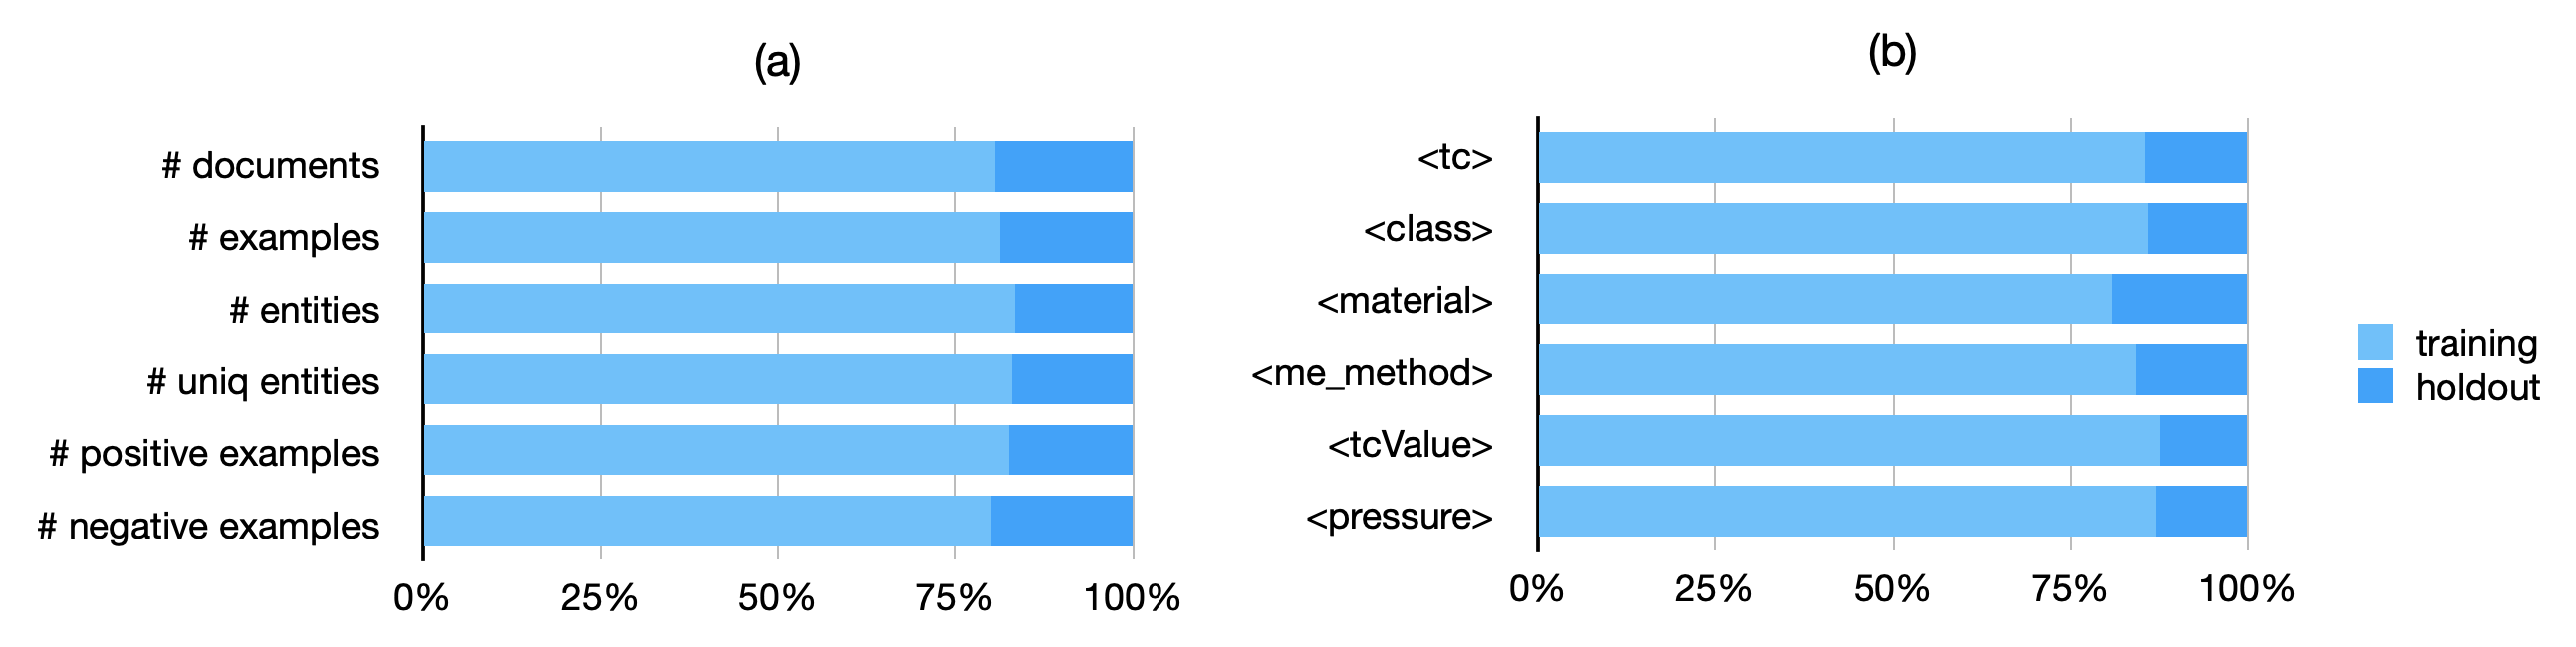
\includegraphics[width=\textwidth]{holdout-training-set}
\caption{Holdout/Training set distribution (a) general metrics and (b) entities labels.
\textit{\# entities} and \textit{\# unique entities} indicate the number of labelled entities with and without value duplicates, respectively. \textit{positive examples} (+) indicates the number of sentences with at least one entity and \textit{negative examples} (-) the number of sentences with no entities.}
\label{fig:training-holdout-set-distribution}
\end{figure}

\begin{figure}[ht]
\centering
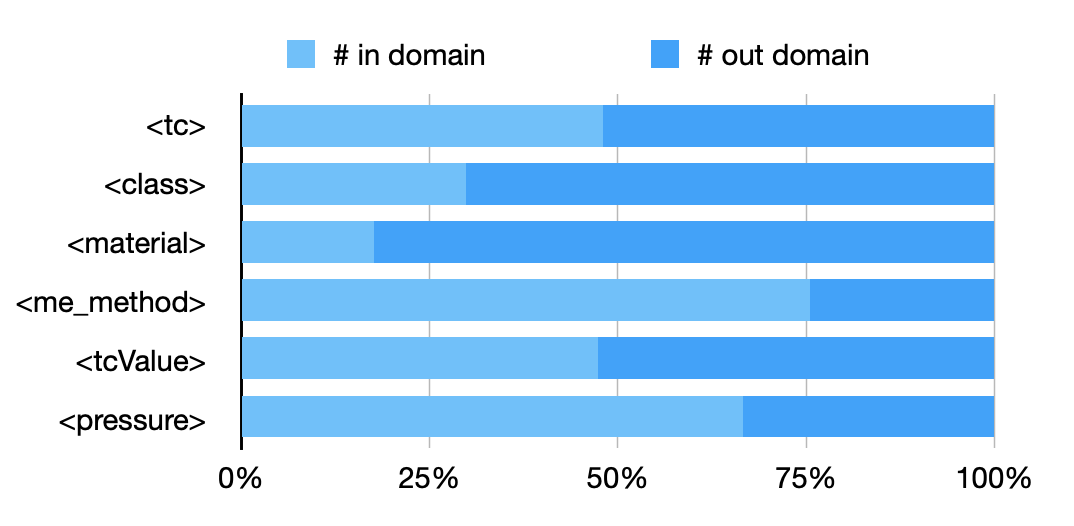
\includegraphics[width=0.6\textwidth]{out-domain-holdout-unique}
\caption{Holdout ``out-of-domain'' rates. Compares the amount of entities from the holdout set that are also in the training set (in-domain) with the entities that are not in the training set (out-of-domain)}
\label{fig:out-domain-holdout}
\end{figure}

\subparagraph*{Positive sampling} 
We train the model with positive sampling by removing the examples without entities (negative examples, Figure~\ref{fig:training-holdout-set-distribution}a). 
Compared with no sampling, this approach provides an improvement by +2\% in both precision and recall, when testing against the holdout set. 
Further experiments with active and random sampling with 0.1, 0.25, 0.5 and 1.0 ratio of negative examples~\cite{lopez2021mining} did not provide stable evidence suggesting improvements for our task. 

\subparagraph*{Evaluation}

We report the evaluation results in Table~\ref{tab:evaluation-superconductors-ML-model}. 
The best results were obtained by Scibert with an F1 of 77.03\%, and recall of around 80.69\%. 
The features did not provide any improvements with RNN models: BidLSTM\_CRF and BidLSTM\_CRF\_FEATURES resulted in the same F1 score.
This result comes as a surprise because features such superscript/subscript were expected to be determinants for recognising materials sequences. 

The \texttt{<pressure>} label obtained the lowest performances for all architectures, we believe 274 training examples are not sufficient considering that pressure expressions can be dependent from the context because they refer to outher type of pressures (e.g. annealing pressure).
The labels with the highest score is \texttt{<material>}, with F1 of 80.77\% and 78.06\% for Scibert and BidLSTM\_CRF, respectively. However, taking in account that such label has the highest ``out-of-domain'' ratio in the holdout set (above 75\%, see Figure~\ref{fig:out-domain-holdout}) and the highest ``label variability'' (the ratio between unique entities and total entities, around 42\%) this suggests that the model can cover well materials that has not been seen in the training. 
On the other hand the \texttt{<me\_method>} label, which has lower ``label variability'' (around 11\%) and low ``out-of-domain'' ratio, obtains an F1 score of 66.56\% with Scibert and 65.92\% with BidLSTM\_CRF.
Surprisingly, for label \texttt{<tc>}, the CRF is outperforming all the other architectures (F1 score of 83.96\%), especially Scibert, which is down to 5 percentage points (78.35\%). We can explain results by pointing out the extremely low variability (12.69\%) of entities labelled as \texttt{<tc>} which is a more favourable terrain for the CRF. %, and having the holdout set with a balanced average ``out-of-domain'' ratio 51\%. 
% The entity labels variability (ratio of unique entities versus the total) is, in average, around 55\%, and 57\% for the training and holdout sets, respectively. \texttt{<tc>} (12\%) and \texttt{me\_method} have the lowest variability while the \texttt{<material>} has the highest. 

Scibert also shows good generalisation capacity for unseen examples or examples appearing in a different context. 
In Figure~\ref{fig:example-comparison-architectures}a only Scibert correctly extracts ``above 100K'', while CRF miss it completely and BidLSTM\_CRF misses ``above''. 
In the training data ``above 100K'' is not present, however, we have ``below 100K'' and ``\~100K'', and we have several other entities containing the token ``above'': ``above 30K'', ``above 2K'', etc. 
Scibert can understand that the token ``above'' is somehow relevant to the temperature. 
In Figure~\ref{fig:example-comparison-architectures}b only Scibert can correctly extract ``W-C nanowire'' that is not present in the SuperMat training data (``out-of-domain'' entity). 
Unfortunately, we cannot check whether ``above 100K'' or ``W-C nanowire'' are also present in the dataset used for pre-train SciBERT by their authors~\cite{Beltagy2019SciBERT} because are not available. 

\begin{figure}[ht]
\centering
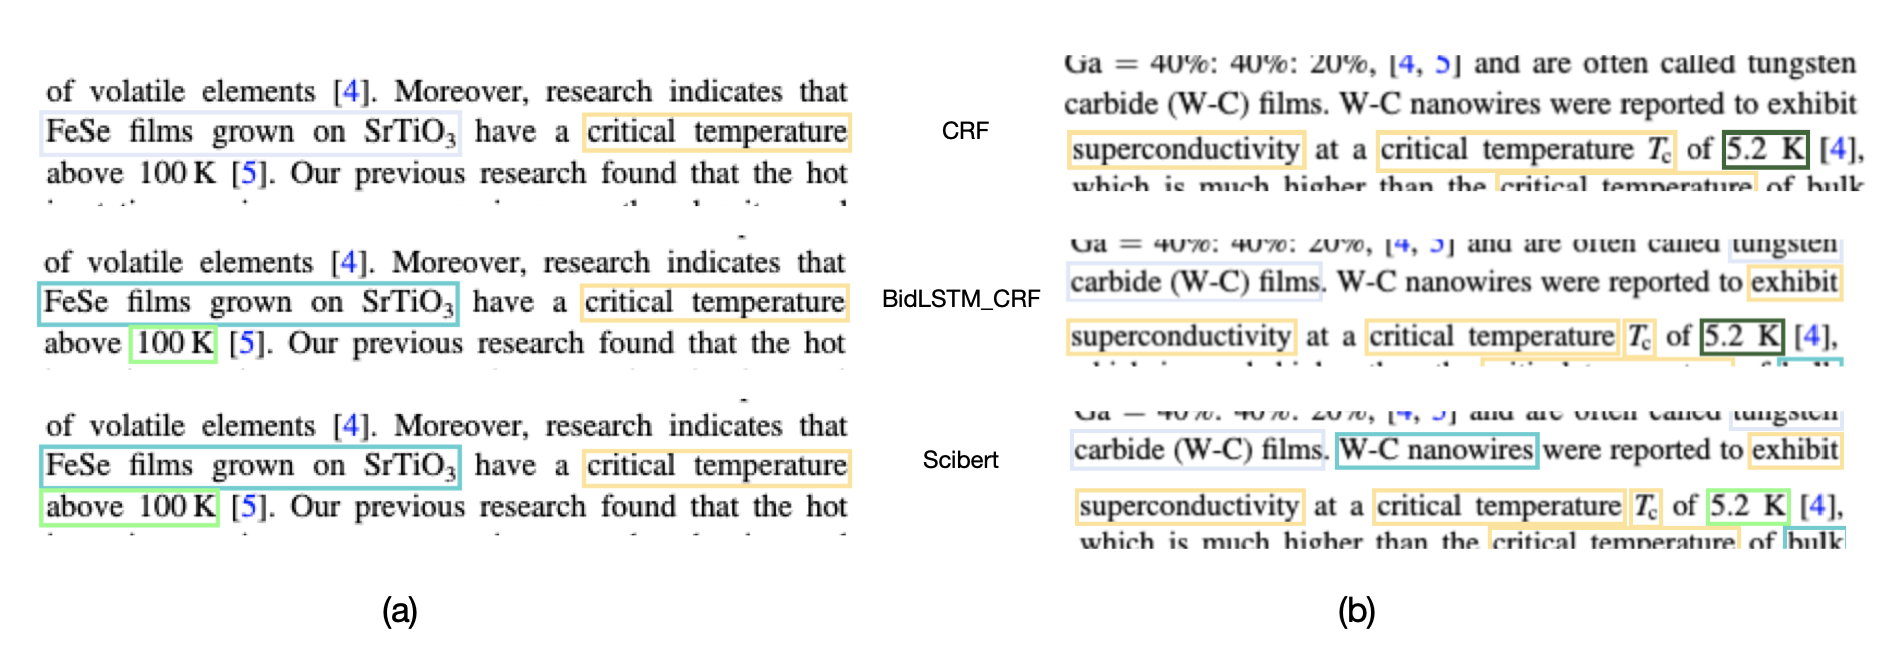
\includegraphics[width=\textwidth]{example-comparison-archs.png}
\caption{Examples~\cite{Gajda_2016, Shibata_2016} of results from different architectures: CRF, BidLSTM\_CRF and, Scibert}.
\label{fig:example-comparison-architectures}
\end{figure}

\begin{table}[ht]
\centering\small
\scalebox{0.66}{
\begin{tabular}{l ccc ccc ccc ccc r}
\toprule
\textbf{Label} & \multicolumn{3}{c}{\textbf{CRF}} & \multicolumn{3}{c}{\textbf{BidLSTM\_CRF}} & \multicolumn{3}{c}{\makecell{\textbf{BidLSTM\_CRF}\\\textbf{\_FEATURES}}} & \multicolumn{3}{c}{\textbf{Scibert}} & \textbf{Supp} \\ 
\cmidrule(lr){2-4}\cmidrule(lr){5-7}\cmidrule(lr){8-10}\cmidrule(lr){11-13}\cmidrule(lr){14-14}  
 & \textbf{P} & \textbf{R} & \textbf{F1} & \textbf{P} & \textbf{R} & \textbf{F1} & \textbf{P} & \textbf{R} & \textbf{F1} & \textbf{P} & \textbf{R} & \textbf{F1} & \\
\midrule
\texttt{<class>}         & 79.74 & 66.79 & 72.69 & 79.01 & 72.62 & \textbf{75.66} & 77.84 & 72.40 & 74.97 & 72.95 & 75.28 & 74.09 & 1646\\
\texttt{<material>}      & 79    & 72.15 & 75.42 & 79.25 & 76.94 & 78.06 & 81.07 & 75.10 & 77.94 & 80.15 & 81.42 & \textbf{80.77} & 6943\\
\texttt{<me\_method>}    & 60.25 & 68.73 & 64.21 & 56.41 & 79.49 & 65.92 & 55.86 & 80.45 & 65.90 & 56.26 & 81.52 & \textbf{66.56} & 1883\\
\texttt{<pressure>}      & 46.15 & 29.27 & 35.82 & 49.45 & 58.05 & 52.53 & 50.25 & 60.49 & \textbf{54.36} & 41.72 & 52.68 & 46.51 & 274\\
\texttt{<tc>}            & 84.36 & 83.57 & \textbf{83.96} & 78.61 & 82.54 & 80.48 & 79.19 & 82.07 & 80.60 & 74.46 & 82.66 & 78.35 & 3741\\
\texttt{<tcValue>}       & 69.8  & 66.24 & 67.97 & 70.36 & 75.16 & 72.67 & 68.95 & 76.56 & 72.52 & 70.90 & 79.74 & \textbf{75.06} & 1099\\
\midrule    
All (micro avg) & 76.88 & 72.77 & 74.77 & 74.59 & 77.67 & 76.09 & \textbf{75.17} & 76.79 & 75.96 & 73.69 & \textbf{80.69} & \textbf{77.03}\\
\bottomrule
\end{tabular}
}
\caption{\label{tab:evaluation-superconductors-ML-model} Evaluation scores for the superconductor ML model in the four architectures. For DL architecture the results are average over 5 runs. Support (Supp) indicate the number of labels in the training data. }
\end{table}

\paragraph*{Material ML model}

To train the \textit{material ML model} we create a special dataset with an additional layer of labels (Table~\ref{tab:material-parser-entities}) having as input the material information represented by entities annotated as \texttt{<material>} in the SuperMat documents.
% (label \texttt{<material>} from \textit{superconductors ML model}, Table~\ref{tab:superconductors-parser-entities}), that is,

\subparagraph*{Holdout set}
The annotations are performed on smaller chunks of text and the throughput is largely higher than the initial effort to develop SuperMat therefore we created an independent holdout set. 
We used material data extracted from a dataset of 500 documents (500-papers) from three publishers: \textit{American Institute of Physics} (AIP), \textit{American Physical Society} (APS) and \textit{Institute of Physics} (IOP)~\cite{foppiano2019proposal}.
The resulting holdout set has a average coverage above 25\% (Figure~\ref{fig:material-training-holdout-set-distribution}) and an ``out-of-domain'' ratio in average of 83.93\% (Figure~\ref{fig:material-out-domain-holdout}). 

\begin{figure}[ht]
\centering
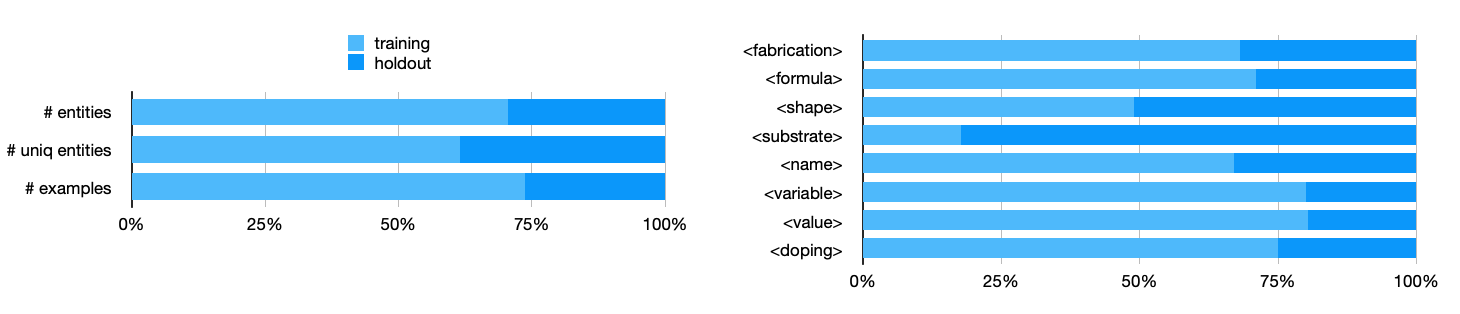
\includegraphics[width=\textwidth]{material-holdout-training-set}
\caption{Holdout/Training set distribution for the \textit{material ML model}. (a) general metrics and (b) entities labels.}
\label{fig:material-training-holdout-set-distribution}
\end{figure}

\begin{figure}[ht]
\centering
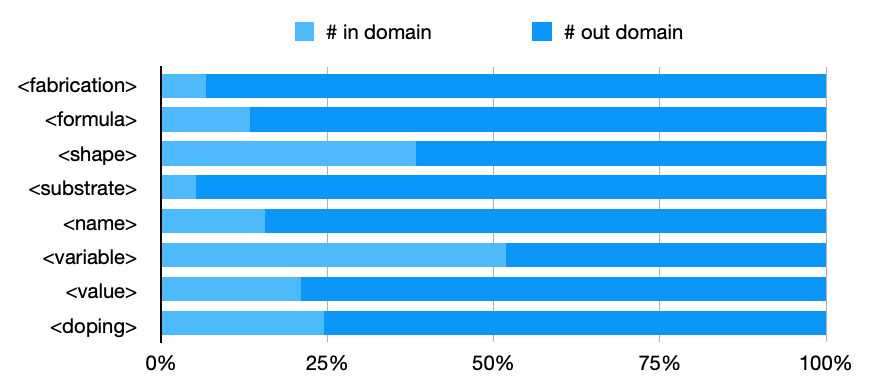
\includegraphics[width=0.6\textwidth]{material-out-domain-holdout-unique}
\caption{Holdout ``out-of-domain'' rates for the \textit{material ML model}. Compares the amount of unique entities from the holdout set that are also in the training set (in-domain) with the entities that are not in the training set (out-of-domain)}
\label{fig:material-out-domain-holdout}
\end{figure}

\subparagraph*{Evaluation}

The results shown in Table~\ref{tab:evaluation-10fold-material-parser} indicate that Scibert obtains the best results, with F1 at 84.15\%.
We confirm for this model that features can be ignored with the BidLSTM\_CRF architecture, they improve the results by less than 1\% (from 83.13 to 83.76\%). 
The label \texttt{<fabrication>} does not perform well with any architecture, we believe, because it is too generic (Table~\ref{tab:material-parser-entities}) and the content is too heterogeneous. Another label, \texttt{<substrate>} has 1/3 of the training examples of \texttt{<fabrication>} but obtains results 3 times higher with Scibert. 
This suggests to split \texttt{<fabrication>} into separate and more homogeneous labels. 

\begin{table}[ht]
\centering\small
\scalebox{0.66}{
\begin{tabular}{l ccc ccc ccc ccc r}
\toprule
\textbf{Label} & \multicolumn{3}{c}{\textbf{CRF}} & \multicolumn{3}{c}{\textbf{BidLSTM\_CRF}} & \multicolumn{3}{c}{\makecell{\textbf{BidLSTM\_CRF}\\\textbf{\_FEATURES}}} & \multicolumn{3}{c}{\textbf{SciBERT}} & \textbf{Supp}  \\
\cmidrule(lr){2-4}\cmidrule(lr){5-7}\cmidrule(lr){8-10}\cmidrule(lr){11-13}\cmidrule(lr){14-14}
 & \textbf{P} & \textbf{R} & \textbf{F1} & \textbf{P} & \textbf{R} & \textbf{F1} & \textbf{P} & \textbf{R} & \textbf{F1} & \textbf{P} & \textbf{R} & \textbf{F1} & \\
\midrule
\texttt{<doping>}      & 60.41 & 55.85 & 58.04 & 67.98 & 62.42 & 64.95 & 69.00 & 62.34 & \textbf{65.43} & 63.58 & 62.79 & 63.16 & 792  \\
\texttt{<fabrication>} & 40.00 & 4.55  & 8.16  & 23.61 &  5.91 &  9.24 & 37.33 &  9.09 & 14.48 & 22.51 & 13.18 & \textbf{16.52} & 94  \\
\texttt{<formula>}     & 80.81 & 82.29 & 81.54 & 82.59 & 84.14 & 83.35 & 83.83 & 85.14 & 84.47 & 84.53 & 86.56 & \textbf{85.53} & 6301\\
\texttt{<name>}        & 72.2  & 63.75 & 67.71 & 76.29 & 78.76 & 77.43 & 74.51 & 80.38 & 77.33 & 77.18 & 81.86 & \textbf{79.44} & 1930 \\
\texttt{<shape>}       & 90.89 & 92.51 & 91.69 & 90.93 & 95.79 & \textbf{93.29} & 90.33 & 95.74 & 92.96 & 89.67 & 97.20 & 93.28 & 809 \\
\texttt{<substrate>}   & 37.04 & 6.76  & 11.43 & 54.31 & 32.43 & 40.44 & 60.08 & 33.38 & 42.82 & 56.32 & 41.22 & \textbf{47.59} & 32 \\
\texttt{<value>}       & 80.21 & 83.15 & 81.65 & 84.81 & 89.33 & 86.99 & 85.16 & 90.15 & \textbf{87.58} & 83.14 & 85.92 & 84.50 & 1895 \\
\texttt{<variable>}    & 96.85 & 95.98 & 96.41 & 95.19 & 97.77 & 96.46 & 96.32 & 97.90 & \textbf{97.10} & 96.22 & 96.52 & 96.37 & 1795 \\
\midrule
All (micro avg)       & 81.15 & 78.09 & 79.59 & 82.76 & 83.50 & 83.13 & \textbf{83.20} & 84.33 & 83.76 & 83.11 & \textbf{85.23} & \textbf{84.15} &   \\
\bottomrule
\end{tabular}
}
\caption{\label{tab:evaluation-10fold-material-parser} Evaluation scores of the material ML model with holdout set. }
\end{table}

\subsection{Entity Linking}
\label{subsubsec:linking}

%Introduction of the linking
The ``Linking'' aims to perform entity linking (EL) between materials and their corresponding properties.
%Objective of the linking
% We can formalised it as follows. \textit{Given a text T and two or more entities e\textsubscript{1}...e\textsubscript{n} of two types t\textsubscript{1} and t\textsubscript{2}, determine links between entities of type t\textsubscript{1} can be linked to entities of type t\textsubscript{2} .} 

%We have experimented several options: dependency parsing, rule-based, and sequence labelling. 
We use a rule-based algorithm; other approaches such as the use of dependency parsing~\cite{yoshikawa:2017acl, Tiktinsky2020pyBARTES, swayamdipta:17, zhou-zhao-2019-head} were discarded. 
It was difficult to find a suitable dependency parser for scientific texts, and complementary methods based on complex rule sets were needed to compensate for the poor performance of the parser.

We link pair of entities focusing on three types of relationships: 
\begin{itemize}
    \item \textbf{material-tcValue} between material and its corresponding superconducting critical temperature value \tc. 
    \item \textbf{tcValue-pressure} between superconducting critical temperature value and its related critical pressure.
    \item \textbf{me\_method-tcValue} connects the superconducting critical temperature value to its corresponding measurement method.
    % \item \textbf{material-crystal\_structure} link the material with their crystal structure, and 
    % \item \textbf{material-space\_group} to link the material to their space groups.
\end{itemize}

Entities of type \texttt{<tcValue>} are pre-processed thorugh a classifier that establish if they are superconductors critical temperature \tc~or not. 
This rule-based classifier combines the extracted entities of T\textsubscript{c} expressions (label \texttt{<tc>}) with a set of predefined standard terms. 
When a T\textsubscript{c} is not considered a ``superconducting critical temperature'' it is excluded from the list of possible linking candidates. 

The linking rule-based approach works considering two scenarios: a) if entities to be linked have cardinality one in the sentence, they are linked automatically. 
When their cardinality is higher then if the word ``\textit{respectively}'' appears in the sentence, we apply ``order-linking'', otherwise ``distance-linking''. 
For example, the sentence:  
\begin{displayquote}
P-or Ba-122  and Co-doped Ba-122 have lower T c s of about 30 K and 24 K, respectively, which makes helium free operation questionable.
\end{displayquote}
containing the word ``respectively'', and applying ``order-linking'' we obtain: \textit{P-or Ba122} is assigned to \textit{30 K} and \textit{Co-doped Ba-122} to \textit{24 K}.
% Such method is very sensible to missing entities and we try to mitigate such scenario, knowing that nothing can be done when entities are missing in the middle of a sentence. 
% We ensure that missing entities at the boundaries limits the incorrect assignment by reducing the search space as follows: 
% \begin{itemize}
%     \item m entities of label\textsubscript{1} vs n entities of label\textsubscript{2} with $m > n$: we shift the starting point to start at the $m - $n entity
%     \item m entities of label\textsubscript{1} vs n entities of label\textsubscript{2} with $m < n$: we shift the ending point at the n\textsubscript{-1} entity
% \end{itemize}

% For example, the following sentence has three entities of type \texttt{<material>} and \texttt{<tcValue>}: 

The other approach ``distance-linking'' works by defining the distance measurement \textit{d} as a value calculated in numbers of characters between the centroid of each entities. 
Entities surrounded by parenthesis are expanded it to the whole parenthesis and its centroid is updated. 
As an example, in the sentence
\begin{displayquote}
We tested two materials MgB2 (Tc = 39 K) and FeSe (Tc = 16 K).
\end{displayquote}

\texttt{39 K} is closer to \texttt{FeSe} (\textit{d}=10) than to \texttt{MgB2} (\textit{d}=11).
Both temperatures entities are expanded to their containing parenthesis e.g. \texttt{39 K} to \texttt{(Tc = 39 K)} in this case the centre of the entity \texttt{39 K} is shifted toward the left, from the initial value of 38 to 35 and the distance from \texttt{MgB2} is reduced from \textit{d}=11 to \textit{d}=8. 
As a result, the \texttt{MgB2} entities is correctly linked to \texttt{39 K}. 

The distance calculation is also adjusted with the addition of ``penalties'' by doubling the calculated distance when certain keywords such as ``,'', ``.'', ``;'', ``and'', ``but', ``while', ``whereas', ``which'', ``although'' representing logical separation of predicates appear between the two entities~\cite{oka2021table}. 
In the above example, the distance between \texttt{39 K} and \texttt{FeSe} will be doubled (\textit{d}=20).

The rule-based linking is evaluated using the linked entities from SuperMat~\cite{foppiano2021supermat} (Table~\ref{table:evaluation-linking}). 
Each task aims evaluating the linking between two entities types, assuming a 100\% accuracy in the previous step. 
The result of the \texttt{material-tcValue} indicates F1 score around 80\% with a precision of 88.40\%.

\begin{table}[ht]
\centering\small
\begin{tabular}{lcccc}
\toprule 
\textbf{Link type} & \textbf{Precision} & \textbf{Recall} & \textbf{F1-score} & Support \\ 
\midrule
\textbf{material-tcValue}      &  88.40    & 74.52 &    80.87 &   726  \\
\textbf{tcValue-pressure}      & 85.71  &  71.52  &  77.98  &  118     \\
\textbf{me\_method-tcValue}    & 62.28 & 65.74 &  63.96  &  151 \\
% \textbf{material-\tc} (CRF)    & 68.52 &	70.11   &  69.16  &  \\
% \textbf{\tc-pressure} (CRF)    & 72.92 &	67.67   &  69.76  &  \\
% \textbf{\tc-me.method} (CRF)   & 49.99 &	45.21   &  44.65  & \\
\bottomrule
\end{tabular}
\caption{\label{table:evaluation-linking} Evaluation scores for the Linking. }
\end{table}

% \subsubsection{Sequence labelling linking} 
% We designed the linking based on sequence labelling as a simple task where each token can be assigned two labels: \texttt{<link\_left>} or \texttt{<link\_right>}. 
% Furthermore, a decoder processing the labelled sequence is assigning links to entities.
% We trained three models, one model for each link type (or entity class pair), using SuperMat~\cite{foppiano2021supermat}.
% The evaluation was performed using 10-fold cross-validation (Table~\ref{tab:evaluation-crf-linking-cross-validation}) with F1 score of 69.16\% for material-tcValue, 44.65\% for tcValue-pressure and 69.66\% for tcValue-me\_method. 

% \begin{table}[ht]
% \centering\small
% % \scalebox{0.7}{
% \begin{tblr}{lrrrr}
% \hline[0.75pt,solid]
% \textbf{Label} & \textbf{Precision} & \textbf{Recall} & \textbf{F1} & \textbf{Support}\\ 
% \hline
% \multicolumn{5}{l}{\hspace{1em}\emph{material-tcValue}} \\
% \hline[dashed]
% \texttt{<link\_left>}  & 70.78   & 73.97 & 72.1  & 505    \\
% \texttt{<link\_right>} & 66.26   & 66.26 & 66.12 & 507    \\
% \hline
% all (micro avg.)       & 68.52   & 70.11 & 69.16 &       \\
% \hline
% \multicolumn{5}{l}{\hspace{1em}\emph{tcValue-me\_method}} \\
% \hline[dashed]
% \texttt{<link\_left>}  & 50.67   & 58.08 & 51.1  & 40    \\
% \texttt{<link\_right>} & 44.71   & 31.83 & 35.68 & 39    \\
% \hline
% all (micro avg.)       & 49.99   & 45.21 & 44.65 &       \\
% \hline
% \multicolumn{5}{l}{\hspace{1em}\emph{tcValue-pressure}} \\
% \hline[dashed]
% \texttt{<link\_left>}  & 76.48   & 67.78  & 70.66 & 113    \\
% \texttt{<link\_right>} & 71.02   & 67.57  & 68.89 & 117    \\
% \hline
% all (micro avg.)       & 72.92   & 67.67  & 69.76 &       \\
% \hline[0.75pt,solid]
% \end{tblr}
% % }
% \caption{Evaluation of the CRF-based linking using 10-fold cross-validation for the three linking models. }
% \label{tab:evaluation-crf-linking-cross-validation}
% \end{table}

% This approach has a several limitations which impact effectiveness in training and tagging. 
% Firstly, since the sequence is flat, (a) it is limited to pairs of adjacent entities. Secondly, (b) the decoding of the annotated sequence is challenging and the linking will not be successful if the sequence of ``right-left'' labels goes out of sync e.g. if the model tags two subsequent entities with the same label one needs to be ignored. Finally, (c) this architecture limit the benefit of the training data, because it supports only certain type of sequences with adjacent entities. The model for tcValue-me\_method is particularly impacted by this limitation because the method of measurement is discussed often far from the actual results are illustrated. 


\subsection{End to end evaluation}

% What is the end 2 end evaluation? 
The end-to-end evaluation (E2EE) measures the capacity of the system on unseen documents.
We limit the scope of the E2EE to the triplet `material-Tc-pressure' which, at the moment, are the backbone upon which the database is built.
We perform the E2EE on the 500-papers dataset where we manually examine the resulting database as follows: a) we mark invalid records and b) we identify the cause of failure from a predefined set of five \textit{error types} (Figure~\ref{fig:error-types}):  
\begin{itemize}
    \item \textbf{From table}: the extracted text is wrongly extracted from a table. Although table content is ignored, the error rate from the Grobid library is still relevant due to the lack of training data. 
    \item \textbf{Extraction}: the failure was caused by entities not recognised, wrongly or partially recognised.
    \item \textbf{Quantities extraction}: the entities of type quantities (pressure, temperature) are not correctly extracted. We measured it separately to identify a failure on a separate ML model.  
    \item \textbf{Tc classification}: the temperature is wrongly classified as superconducting Tc
    \item \textbf{Linking}: given the precedent steps were performed correctly, the resulting entities were not linked correctly. 
\end{itemize}

\begin{figure}[ht]
\centering
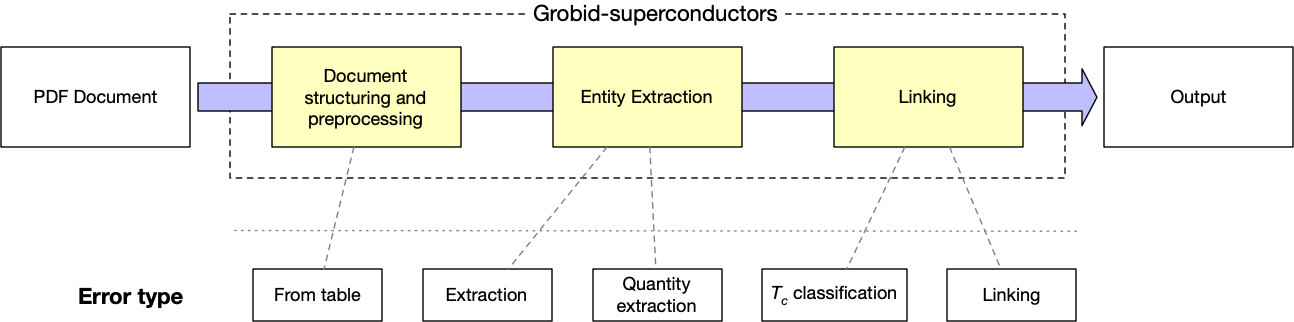
\includegraphics[width=\textwidth]{error-types-colors}
\caption{\textit{Error types} in the context of the data flow. }
\label{fig:error-types}
\end{figure}

The E2EE scores are illustrated in (Table~\ref{table:end2end-evaluation-summary}). 
The recall is omitted because less relevant and difficult to calculate manually. 
The system scores 72.60\% precision considering all the subsections. 
Comparing precision by subsection, we notice a clear difference between the error rates of Figure caption (59.28\%) and unknown subsections (57.14\%) with the rest of the other subsections ($>$ 70\%). 
Unknown\textit{subsections} indicate that the extracted text was not well identified by Grobid but it was aggregated nevertheless.
The scores increase to 73\% when excluding unknown subsections, 75.24\% when excluding figure captions, and 79.14\%  when excluding both. 
Excluding these two subsections will not impact the amount of text, because both count for less than 20\% of the total number of subsections. 


\begin{table}[ht]
\centering\small
\begin{tabular}{l c c}
\toprule
\textbf{Subsection} & \textbf{Precision} & \textbf{Support} \\ 
\midrule
Title               & 100       & 2     \\
Abstract            & 80.32     & 61    \\
Paragraph           & 75.2      & 623   \\    
Figure captions     & 59.28     & 140   \\    
Unknown             & 57.14     & 21    \\
\midrule
\textbf{Micro avg.}  & 72.60     & 847   \\
\textbf{Micro avg.} (excl. figures)  & 75.24     & 707   \\ 
\textbf{Micro avg.} (excl. unknown sections)  & 73.00     & 603   \\ 
\textbf{Micro avg.} (excl. figures and unknown sections)  & 79.14     & 657   \\ 
\bottomrule
\end{tabular}
\caption{Evaluation end to end: summary of the scores. }
\label{table:end2end-evaluation-summary}
\end{table}

The error types are summarised in Figure~\ref{fig:error-types-distribution}. The most common failures  originate from Tc classification (40\%), Linking (32\%), and Extraction (20\%).

\begin{figure}[ht!]
\centering
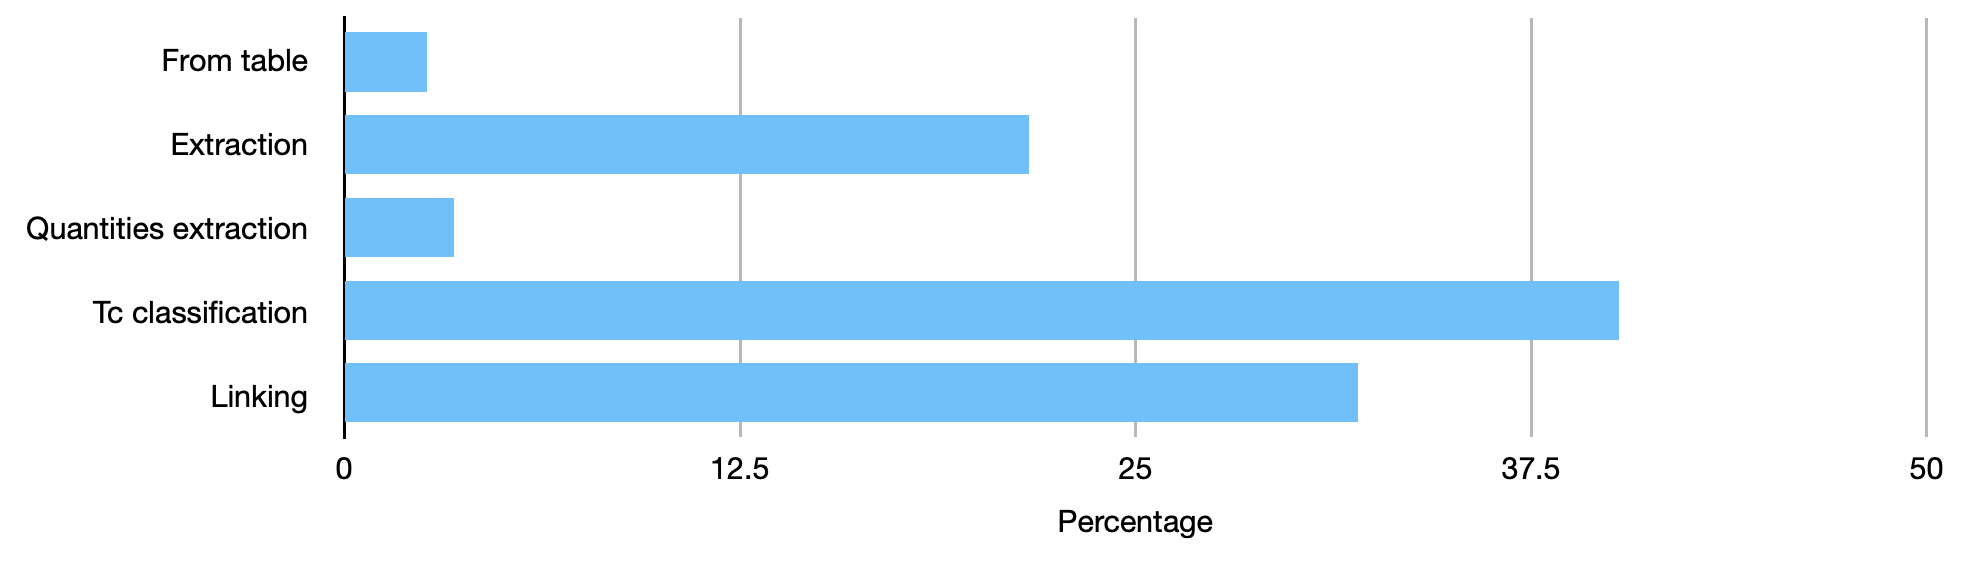
\includegraphics[width=\linewidth]{error-types-bars-perc}
\caption{Error type distribution in the E2EE on the \textit{500-papers} dataset.}
\label{fig:error-types-distribution}
\end{figure}


The most common Tc classification failures are as incorrect recognition of a) relative values of \tc (eg. 1 K higher than material X), b) values indicating the transition temperature width ($\Delta T_{c}$),  c) temperature values that are not \tc, for example, material synthesis temperatures $T$, other critical transition temperatures that are not superconducting (e.g $T_{Curie}$), and d) values of temperature at which there is no superconductivity (e.g at 70 K there is no superconductivity).
The errors of type ``Linking'' occurs mainly when the authors are comparing relative values of \tc~using materials for comparison (e.g. \textit{The Tc = 38 K is similar to the one of MgB$_{2}$}). 
Finally, ``Extraction'' issues originate mainly from: a) implicit mention of the main material when experimented with different substrates, and b) mismatches between \texttt{<material>} and \texttt{<class>} which, by definition, overlap. 

% \begin{table}[ht]
% \centering
% \begin{tabular}{lcc}
% \hline \textbf{Error type} & \textbf{Rate} & \textbf{Support} \\ 
% \hline
% From table              & 2.58  & 6     \\
% Extraction              & 20.25 & 47    \\
% Quantities extraction   & 3.44  & 8     \\
% Composition resolution  & 1.29  & 3     \\
% Tc classification       & 40.08 & 93    \\
% Linking                 & 31.89 & 74    \\
% \hline
% \hline
% \textbf{Total}  & & 231   \\
% \hline
% \end{tabular}
% \caption{Evaluation end to end: error types. }
% \label{table:end2end-evaluation-errur types}
% \end{table}


\section{Supercon\textsuperscript{2}}

We created SuperCon\textsuperscript{2} by processing 37770 research papers belonging to the category \textit{cond-mat.supr-cond} in ArXiv. 
Currently SuperCon\textsuperscript{2} contains 40324 records including 2052 triplets \textit{material-Tc-applied pressure}, and 3602 records with explicit measurement method \textit{material-Tc-measurement method}.
% The schema contains additional information which are described in Table~\ref{tab:superconductors-parser-entities} and~\ref{tab:material-parser-entities} and richer bibliographic data described in Section~\ref{subsubsec:document-structuring}. 
The schema of SuperCon\textsuperscript{2} is summarised with examples in Table~\ref{tab:supercon2-schema}. 


\afterpage {
    \clearpage % Flush earlier floats (otherwise order might not be correct)
    
\begin{table}[ht]
\centering\small
\scalebox{0.8}{
\begin{tblr}{Q[l,m]Q[r,m]Q[r,m]}
\hline[1pt]
\textbf{Field name} & \textbf{Description} & \textbf{Examples} \\ 
\hline
\multicolumn{3}{c}{\emph{Material information}} \\
\hline[dashed]
{Raw\\ material} & The material or sample as it appears in the text &\\
\hline[dotted]
Name  & Canonical name of a material & {PCCO, PCO, Metal diboride,\\ hydrogen, carbon} \\
\hline[dotted]
Formula & {Material expressed as chemical formula. This\\ includes also formulas with stochiometric variables} & {$Pr_{1.869}Ce_{0.131}CuO_4-\delta$,\\ $MgB_2$, $La_{2-x} Sr_x CuO_4$} \\
\hline[dotted]
Doping  & {Doping ratio and doping materials\\ that might be adjointed to the material} & {Overdoped, underdopded,\\ optimally doped,\\ bulk, pure, 1\% Zn, Zn\\ (from Zn-doped XYZ)}\\
\hline[dotted]
Shape  & The shape of the material or the sample & {Single crystal, polycrystal,\\ wire, powder, film} \\
\hline[dotted]
Variables  & Variables that can be substituted in the formula & x = 0, RE=Ln,St\\
\hline[dotted]
Class  & {Material classification according\\ to the domain-experts taxonomy} & cuprates, oxides, alloys\\
\hline[dotted]
Fabrication  & {All the information that does not\\ belong to any of the previous tags} &  {Intercalated,\\ synthesized by MBE method,\\ electron-doped, hole-doped} \\
\hline[dotted]
Substrate  & Substrate material described in the raw material & {PCCO films onto\\ $Pr_2 CuO_4 (PCO)/SrTiO_3$ }\\
\hline[dashed]
\multicolumn{3}{c}{\emph{Properties}} \\
\hline[dashed]
{Critical\\ Temperature}  & Superconducting critical temperature &\\
\hline[dotted]
{Applied \\ Pressure}  & {Pressure applied when measuring \\ the superconducting critical temperature} &\\
\hline[dotted]
{Measurement \\ Method}  & {Method for measurement of the\\ superconducting critical temperature} & {Magnetic susceptibility,\\ specific heat, calculation,\\ prediction, resistivity}\\
\hline[dashed]
\multicolumn{3}{c}{\emph{Document bibliographic information}} \\
\hline[dashed]
Section & The main body section of the paper & Header, body, annex\\
\hline[dotted]
Subsection & The secondary segmentation area of the paper & {Paragraph, table caption,\\ figure caption, title, abstract} \\
\hline[dotted]
{Authors,\\ Title, DOI,\\ Publisher,\\ Journal, Year} & \multicolumn{2}{c}{Bibliographic information of the document}\\
\hline[dashed]
\multicolumn{3}{c}{\emph{Internal information}} \\
\hline[dashed]
                {Hash,                                                                                                 \\ Timestamp} & \multicolumn{2}{c}{Hash calculated on the binary content of the original PDF\\ document and the timestamp when the document was processed.}\\
\hline[1pt]
\end{tblr}
}
\caption{\label{tab:supercon2-schema} Summary and description of the SuperCon\textsuperscript{2} schema. \textit{Internal information} are technical information not accessible to the users.}
\end{table}
    \clearpage 
}


The data is ingested through the asynchronous Map-Reduce approach~\cite{10.1145/1327452.1327492}. 
The ``Extraction task'' processes the PDF documents with \textit{grobid-superconductors} and stores their processed representation together with the original PDF document.
Furthermore, the ``Aggregation task'' reduces the document information in a synthesised tabular format.
We store the processed document representation in JSON format, and they are keep separately to being used for visualisation together with the original PDF. 
The pipeline uses a persistence layer for storage and reporting (logger) accessing \textit{grobid-superconductors} via REST API.  

% \begin{figure}[ht]
% \centering
% 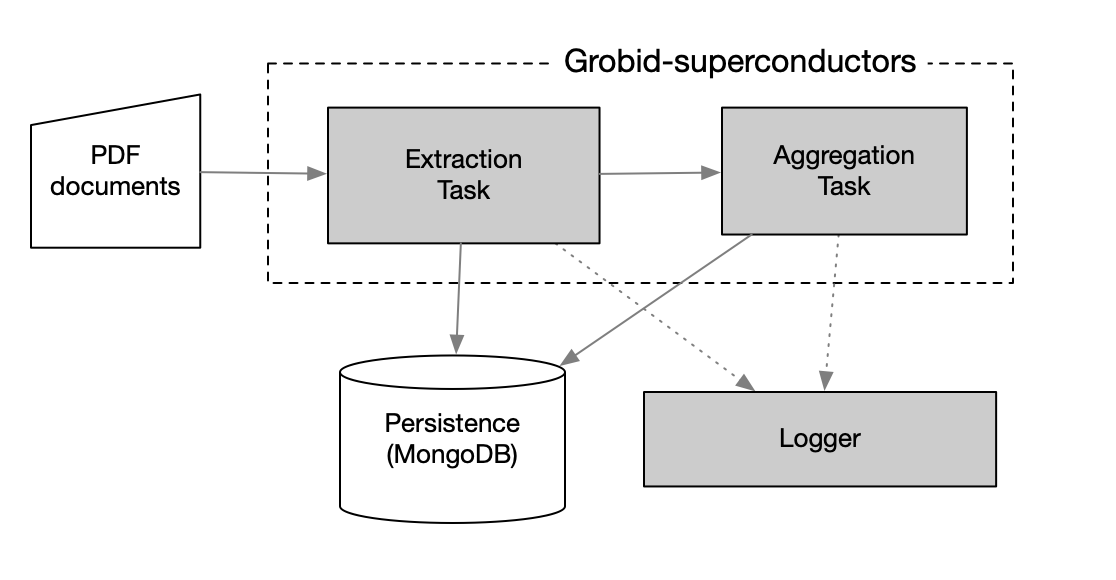
\includegraphics[width=0.7\textwidth]{workflow-schema-1}
% \caption{Schema of the ingestion workflow}
% \label{fig:ingestion-workflow}
% \end{figure}


% \subsection{Curation interface}
% \label{sucsec:supercon2-user-interface}
% SuperCon\textsubscript{2} can be utilised as text file (CSV or TSV) for processing and to build ML models and data-driven applications. 

% Although the automatic system might achieve good results and extract a large quantity of data, we are aware that some sort of ``user validation'' is required for improving the data quality. For this reason we have built SuperCon\textsubscript{2} with in mind the needs of an efficient curation interface. 
We built a visualisation interface to exploit the extracted information. 
Users can search in the synthesised tabular data, access the PDF document enriched with the extracted information (Figure~\ref{fig:pdf-annotations}), and export locally in CSV, TSV and Microsoft Excel formats. 

\begin{figure}[ht!]
\centering
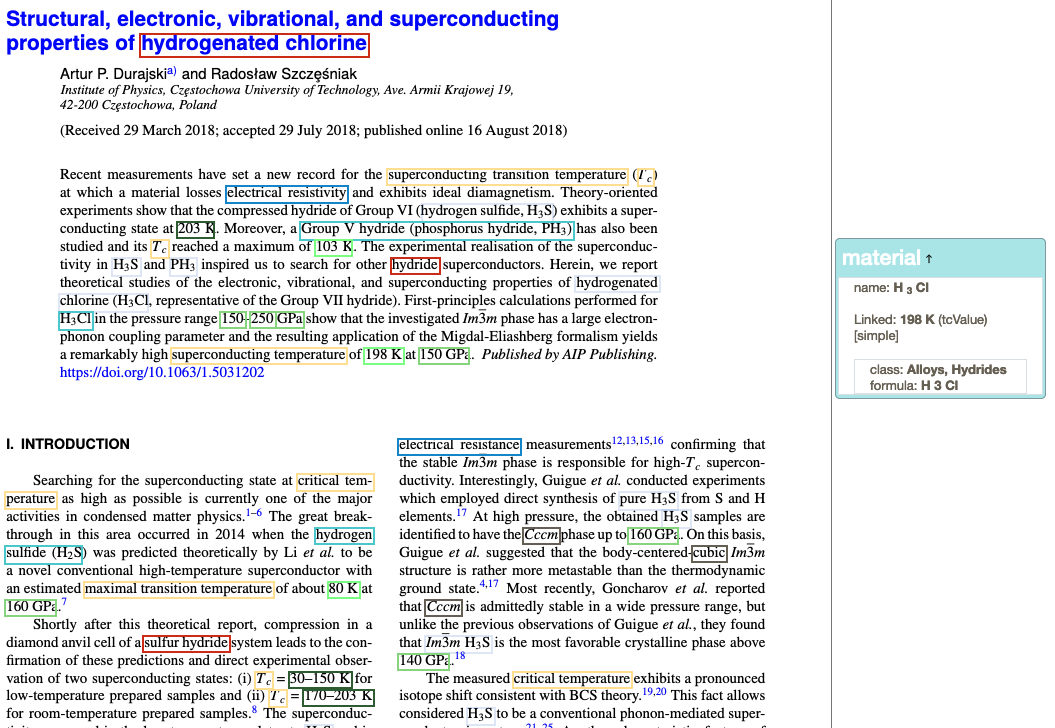
\includegraphics[width=0.8\textwidth]{sample-pdf-annotations}
\caption{\label{fig:pdf-annotations} Example of superconductors research PDF document~\cite{sample_superconductors_article} enriched with extracted annotations. Materials information (class, formula) and properties (\tc) are summarised in the information box when clicking to the highlighted annotated entity in the text.}
\end{figure}

\section{Conclusion}
\label{sec:conclusion}
In this work, we present our solution for automatically building a database of materials and properties from scientific literature. 
Our contribution is composed of: a) \textit{grobid-superconductors}, a specialised open source system that processes PDF documents combining ML and rule-based methods to extract and link relevant information in superconductors research.
b) A pipeline allowing large-scale document processing, and c) a visualisation interface for rapid data exploration which includes PDF documents information enrichment. 

We made SuperCon\textsuperscript{2}, a database with 40324 records of superconductors materials and properties including the applied pressure and the \tc~measurement method. 
SuperCon\textsubscript{2} is available in text format at \url{https://github.com/lfoppiano/supercon}.

In future, we plan to improve our tools by a) extracting more properties, such as crystal structure type, space groups type, and lattice structure, b) train supervised models for the Linking step, and c) extending the interface to support data correction toward efficient curation.
We confirmed the good generalisation ability of the Scibert architecture for NER task in materials science domain. 
There are hopes to obtain better results using materials science pre-trained BERT, such as matscibert~\cite{gupta_matscibert_2022}, however, the gain might be just minimal for relatively larger models~\cite{hong2022ScholarBERT}.

\section*{Acknowledgement}
\label{sec:acknowledgement}
Our warmest thanks to Patrice Lopez, the author of Grobid~\cite{GROBID}, DeLFT~\citep{DeLFT} and many other interesting open-source projects.

%\section*{Notes on contributors}
% for later 


\section*{Competing interests} 

The authors declare no competing interests.


\bibliography{bibliography}
\bibliographystyle{tfnlm}

% \begin{appendices}
\appendix

\section{Dataset additional information}

\begin{table}[ht]
\centering\small
\begin{tabular}{lccc}
\toprule
& \textbf{training}  & \textbf{holdout} & \textbf{holdout/training}      \\
\midrule
\textbf{\# documents}        & 132   & 32    & 24.24\%   \\
\textbf{\# examples}       & 16902 & 3905  & 23.10\%   \\
\textbf{\# entities}        & 15586 & 3112  & 19.97\%   \\
\textbf{\# unique entities} & 6699  & 1372  & 20.48\%   \\
\textbf{\# positive examples}    & 8380  & 1776  & 21.19\%   \\
\textbf{\# negative examples}    & 8522  & 2129  & 24.98\%   \\
\bottomrule

\end{tabular}

\caption{Holdout/Training set distribution between training and holdout sets for the \textit{superconductors ML model}. \textit{\# positive examples} indicate the number of sentences with at least one entity, and \textit{\# negative examples} the number of sentences with no entities.}
\label{tab:training-holdout-set-distribution-annex}
\end{table}

\begin{table}[ht]
\centering\small
\begin{tabular}{lccc}
\toprule
label & \textbf{training}  & \textbf{holdout} & \textbf{holdout/training }     \\
\midrule
\texttt{<tc>}           & 3741      & 639   & 17.08\%   \\
\texttt{<class>}        & 1646      & 271   & 16.46\%   \\
\texttt{<material>}     & 6943      & 1649  & 23.75\%   \\
\texttt{<me\_method>}   & 1883      & 355   & 18.85\%   \\
\texttt{<tcValue>}      & 1099      & 157   & 14.29\%   \\
\texttt{<pressure>}     & 274       & 41    & 14.96\%   \\
\bottomrule

\end{tabular}

\caption{Holdout/Training set distribution between training and holdout sets on different labels for the \textit{superconductors ML model}.}
\label{tab:training-holdout-labels-distribution-annex}
\end{table}

\begin{table}[ht]
\centering\small
\begin{tabular}{lccc}
\toprule
& \textbf{training}  & \textbf{holdout} & \textbf{holdout/training}      \\
\midrule
\textbf{\# examples}        & 13648 & 5728  & 41.97\%   \\
\textbf{\# entities}        & 4512  & 2817  & 62.43\%   \\
\textbf{\# unique entities} & 9268  & 3292  & 35.52\%   \\
\bottomrule

\end{tabular}

\caption{Holdout/Training set distribution training and holdout sets for the \textit{material ML model}.}
\label{tab:training-holdout-set-material-distribution-annex}
\end{table}

\begin{table}[ht]
\centering\small
\begin{tabular}{lccc}
\toprule
label & \textbf{training}  & \textbf{holdout} & \textbf{holdout/training }     \\
\midrule
\texttt{<fabrication>}  & 94    & 44    & 46.81\%   \\
\texttt{<formula>}      & 6301  & 2569  & 40.77\%   \\
\texttt{<shape>}        & 809   & 841   & 103.96\%   \\
\texttt{<substrate>}    & 32    & 148   & 462.50\%   \\
\texttt{<name>}         & 1930  & 949   & 49.17\%   \\
\texttt{<variable>}     & 1795  & 449   & 25.01\%   \\
\texttt{<value>}        & 1895  & 463   & 24.43\%   \\
\texttt{<doping>}       & 792   & 265   & 33.46\%   \\
\bottomrule

\end{tabular}

\caption{Holdout/Training set distribution training and holdout sets on different labels for the \textit{material ML model}.}
\label{tab:training-holdout-labels-material-distribution-annex}
\end{table}


\section{Machine learning support material}

\begin{table}[ht]
\centering\small
\scalebox{0.71}{
\begin{tabular}{l m{30em} c c}
\toprule
\textbf{\#} & \textbf{Feature} & \textbf{Model} & \textbf{Architecture}\\ 
\midrule
\textbf{1} & current token & all & all\\
\textbf{2} & current token lower cased & all & all\\
\textbf{3-6} & (four features) current token, prefix characters 1 to 4 & all & CRF\\
\textbf{7-10} & (four features) current token, suffix characters 1 to 4 & all & CRF\\
\textbf{11} & information about capitalisation: first character (INITCAP), all characters (ALLCAPS), none (NOCAPS) & all & all\\
\textbf{12} & digits content: all (ALLDIGIT), some digits (CONTAINDIGIT), no digits (NODIGIT) & all & all \\ 
\textbf{13} & (boolean) the token is composed by a single character & all & all\\ 
\textbf{14} & punctuaction information and normalisation to placeholders: no punctuation (NOPUNCT), open or end brackets (OPENBRACKET, ENDBRACKET), various punctuation (DOT, COMMA, HYPHEN, QUOTE), open or close quotes (OPENQUOTE, ENDQUOTE), anything else (PUNCT) & all & all\\
\textbf{15} & Shadow the numbers & all & CRF\\
\textbf{16} & Shadow any characters: ``x'' for lowercase, ``X'' for uppercase, ``d'' for digits & all & CRF \\
\textbf{17} & As the previous but compressed & all & CRF\\
\textbf{18} & Font name & superconductors & all\\
\textbf{19} & Font size & superconductors & all\\
\textbf{20} & Font style: standard (BASELINE), superscript (SUPERSCRIPT) or subscript (SUBSCRIPT) & superconductors & all\\
\textbf{21} & (boolean) if the token style is bold  & superconductors & all\\
\textbf{22} & (boolean) if the token style is italic & superconductors & all\\
\textbf{23} & (boolean) the token is identified as a chemical compound by ChemDataExtractor\cite{chemdataextractor}  & superconductors & all\\
\bottomrule
\end{tabular}
}
\caption{Summary of the features used in the \textit{superconductors} and \textit{material} ML models. \textit{All} under Architecture indicate only BidLSTM\_CRF\_FEATURES and CRF.}
\label{tab:ML-model-features}
\end{table}

% \end{appendices}



\end{document}
